\section{Messergebnisse und Auswertung}
\subsection{Fehler der Messgrößen}
In \autoref{tab:errors} sind die hier verwendeten Messgrößen mit ihren Fehlern aufgelistet. Da es zu den verwendeten Geräten von den Herstellern 
keine Angabe des Fehlers gab, sind dies alles geschätzte Werde. Die Fehler des Magnetfeldes und der Stromstärke, mit welcher die magnetfelderzeugenden 
Spulen durchflossen wurden, wurde auf einen Digit-Fehler gesetzt. Der Fehler der Frequenz wurde durch Variation, ohne dass sich das Signal auf dem 
Oszilloskop bemerkbar verändert, bestimmt. Auf die Eindringtiefe wurde ein Fehler einer halben Skalenbreite geschätzt.
\begin{table}[H]
\begin{center}
\begin{tabular}{|l|c|}
  \hline
  \textbf{Messgröße} & \textbf{Fehler} \\ \hline
  Magnetfeld $B$ & 1 mT \\ \hline
  Frequenz $\nu$ & 0.005 MHz \\ \hline
  Eindringtiefe $x$ & 0.5 mm \\ \hline
  Stromstärke $I$ & 0.01 A \\ \hline 
\end{tabular}
\caption{Fehler der Messgrößen}
\label{tab:errors}
\end{center}
\end{table}

\subsection{Vermessung des Magnetfeldes}
\subsubsection{Ortsabhängigkeit}
Die Abhängigkeit der Stärke $B$ des Magnetfeldes von der Eindringtiefe $x$ ist in \autoref{img:B:x} dargestellt. 
Das Magnetfeld ist größtenteils homogen, nur in den Randbereichen fällt es ab. Das Plateau wurde in \autoref{img:B:x:zoom} vergrößert 
dargestellt. Für die folgenden Messungen wurde die Eindringtiefe der Hallsonde und die Position der Proben auf $x=20$\,mm eingestellt.

\begin{figure}[H]
\begin{center}
  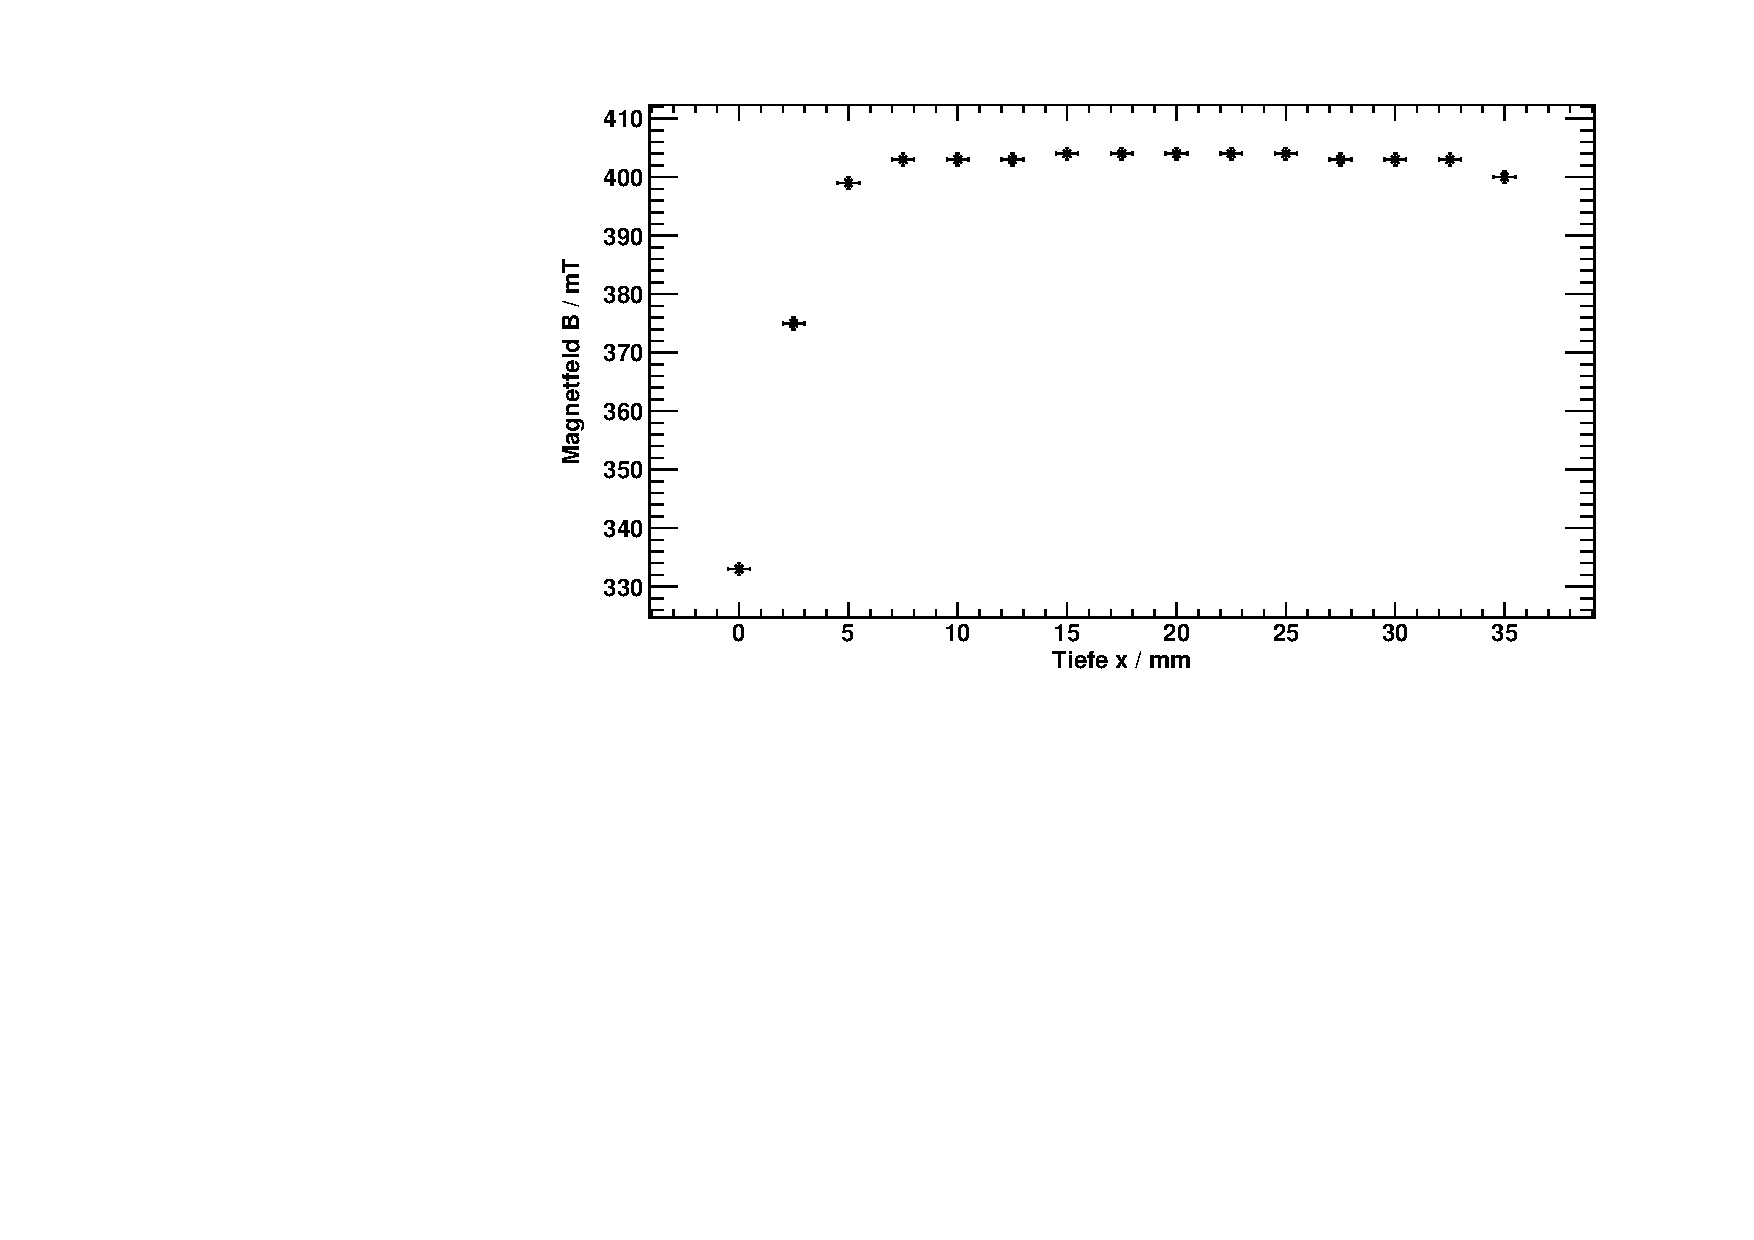
\includegraphics[width=\textwidth]{../img/01-B-x.pdf}
  \caption{Magnetfeldstärke $B$ in Abhängigkeit der Eindringtiefe $x$.}
  \label{img:B:x}
\end{center}
\end{figure}
\begin{figure}[H]
\begin{center}
  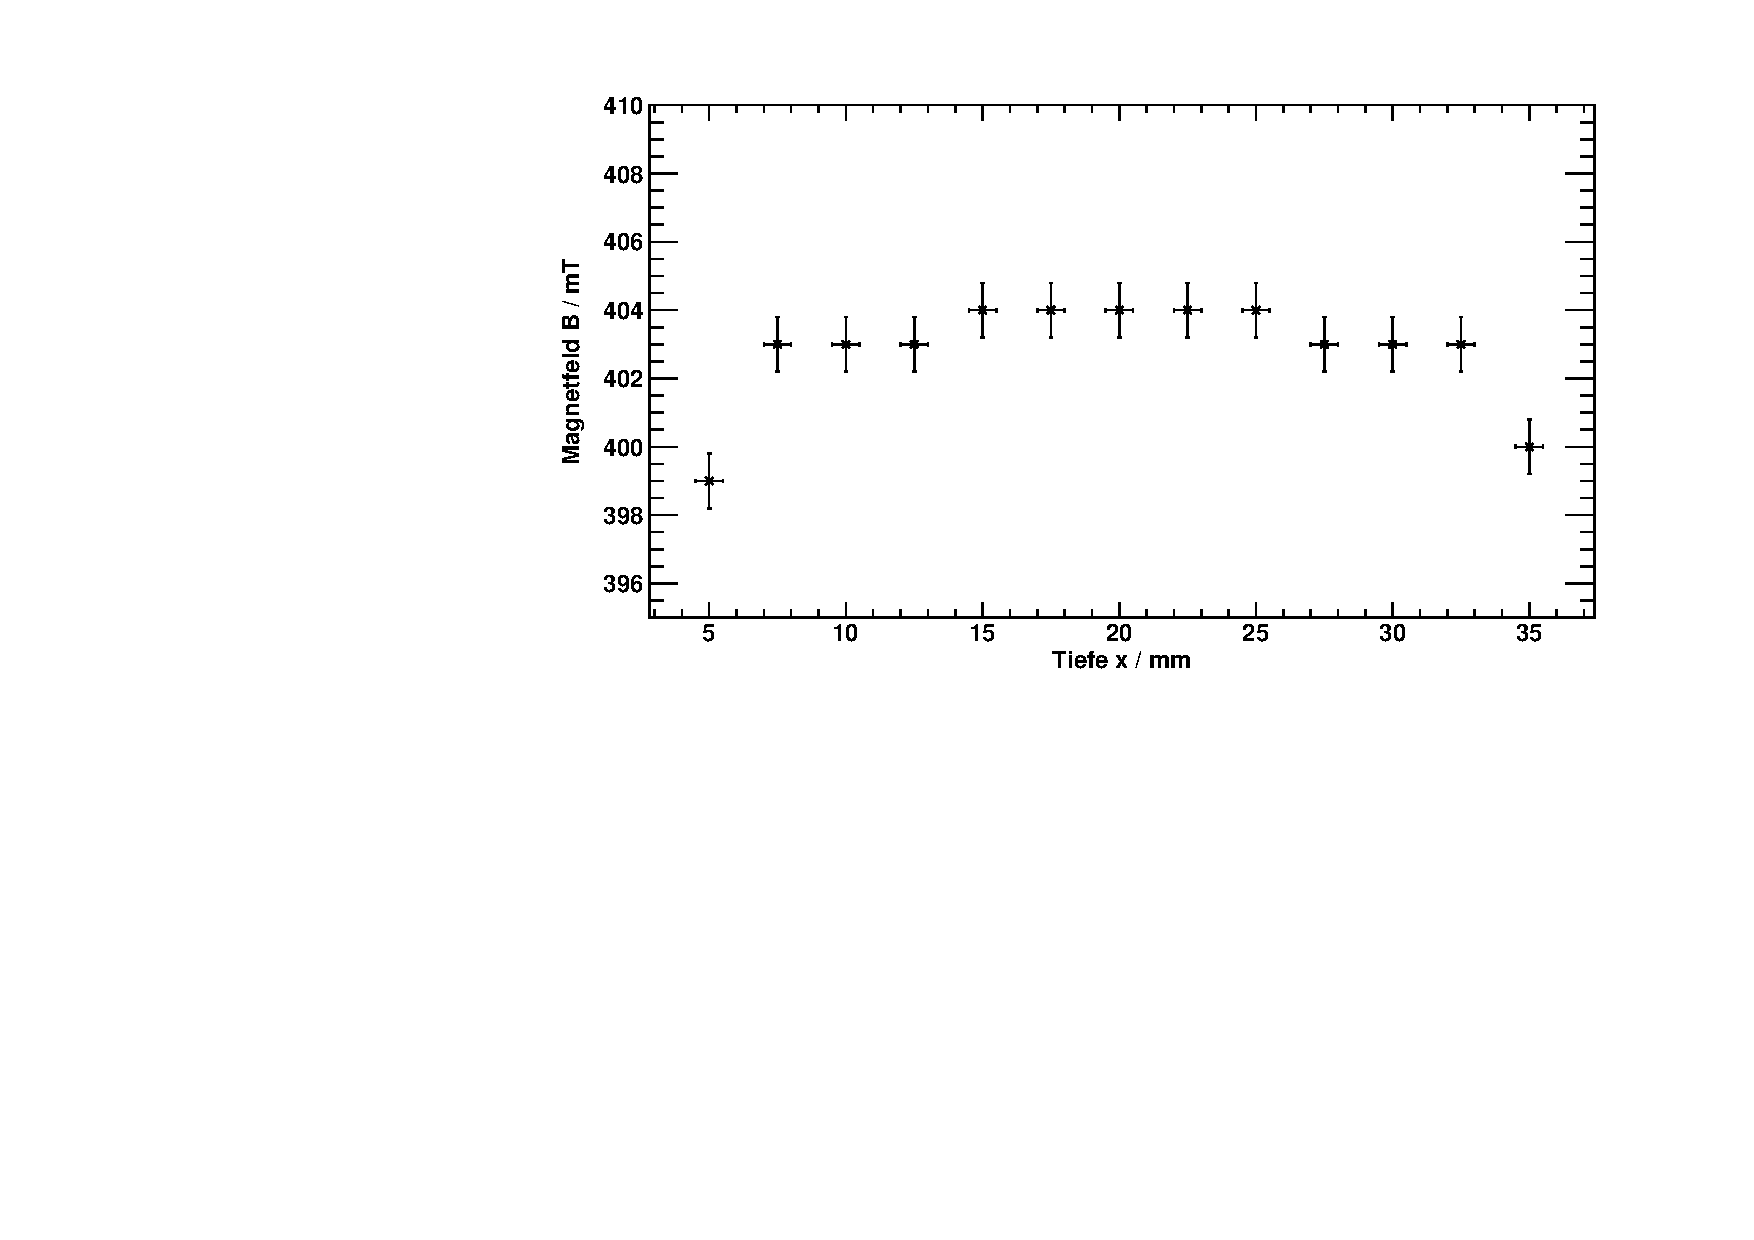
\includegraphics[width=\textwidth]{../img/01-B-x-zoom.pdf}
  \caption{Vergrößerung von \autoref{img:B:x}.}
  \label{img:B:x:zoom}
\end{center}
\end{figure}

\subsubsection{Stromabhängigkeit}
In \autoref{img:B:I} sieht man die Abhängigkeit der Stärke $B$ des Magnetfeldes von dem verwendeten Strom. 
Das Magnetfeld steigt zunächst linear mit dem Strom an, ab 3\,A wird jedoch eine Sättigung bemerkbar. \\
Es wurden zwei Messreihen aufgenommen, die 
sich in der Richtung der Änderung des Stroms unterscheiden. Es lässt sich ein Hystereseffekt erkennen, je nachdem ob vor der aktuellen Messung 
einen höheren oder niedrigeren Strom eingestellt wurde. Dies ist jedoch für die nachfolgenden Messungen und Berechnungen nicht relevant, da direkt 
die Stärke des Magnetfeldes bestimmt wird. Mit dieser Messung konnte die einzustellende Stromstärke für ein bestimmtes Magnetfeld $B$ bei einer 
festgelegten Frequenz $\nu$ geschätzt werden, was die Suche nach dem genauen Wertepaar von $B$ und $\nu$, bei welchem Resonanz beobachtet wird, 
beschleunigt.
\begin{figure}[H]
\begin{center}
  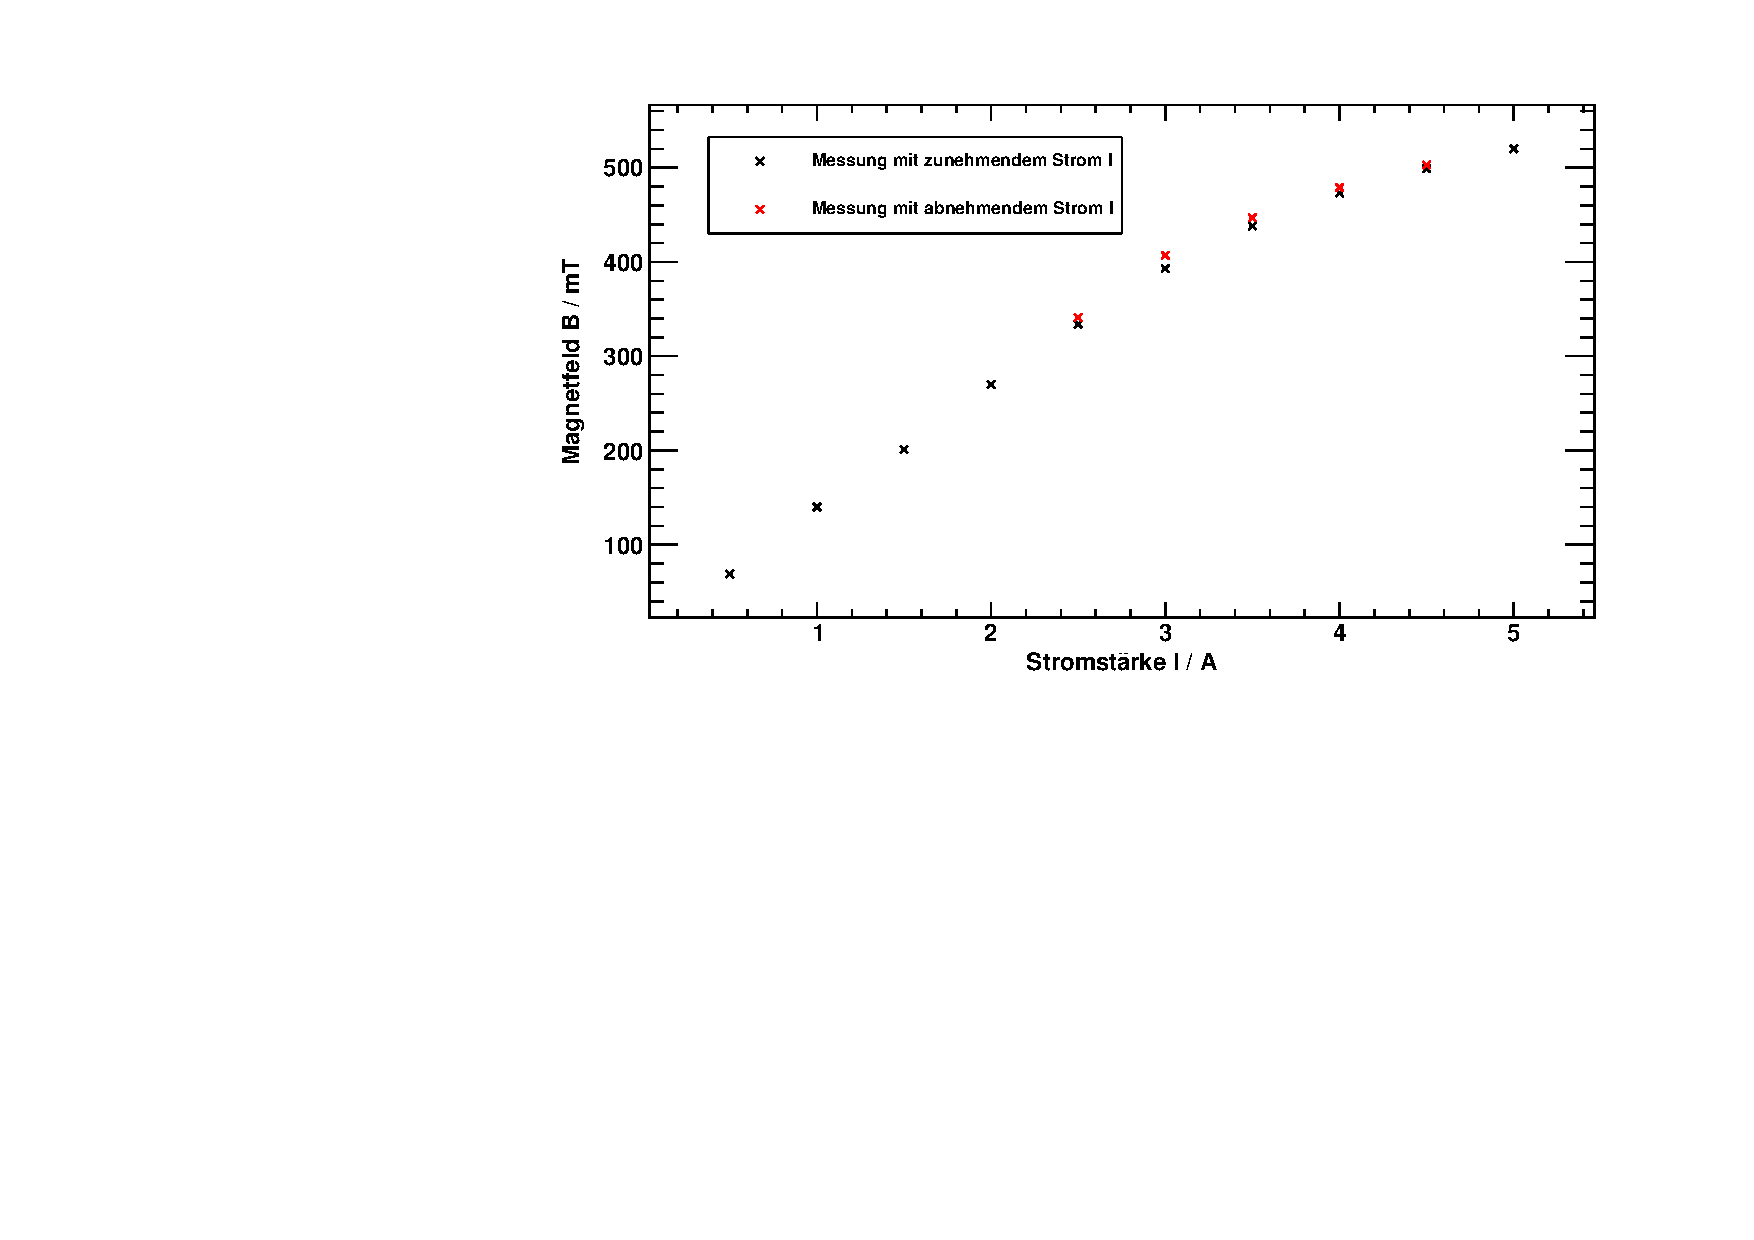
\includegraphics[width=\textwidth]{../img/02-B-I.pdf}
  \caption{Magnetfeldstärke $B$ in Abhängigkeit des Stroms $I$ und Richtung der Veränderung dessen.}
  \label{img:B:I}
\end{center}
\end{figure}

\subsection{Bestimmung der gyromagnetischen Verhältnisse}
Um das gyromagnetische Verhältnis $\gamma$ zu bestimmen, ist im Prinzip genau eine Resonanzfrequenz $\nu$ mit entsprechender Magnetfeldstärke $B$ notwendig. 
Um jedoch den Fehler auf $\gamma$ besser abzuschätzen wurden für Wasserstoffprobe mehrere Messwerte aufgenommen. Aus dem Fit lässt sich auch $\gamma$ 
bestimmten, jedoch lässt sich der Fehler besser abschätzen, da auch statistische Schwankungen berücksichtigt werden. Der relative Fehler des so 
bestimmen Wertes für $\gamma_H$ wird deshalb auch als Fehlern der anderen gyromagnetischen Verhältnisse, berechnet aus nur einem Wertepaar, berechnet.
\subsubsection{Berechnung von $\gamma_H$}
\begin{figure}[H]
\begin{center}
  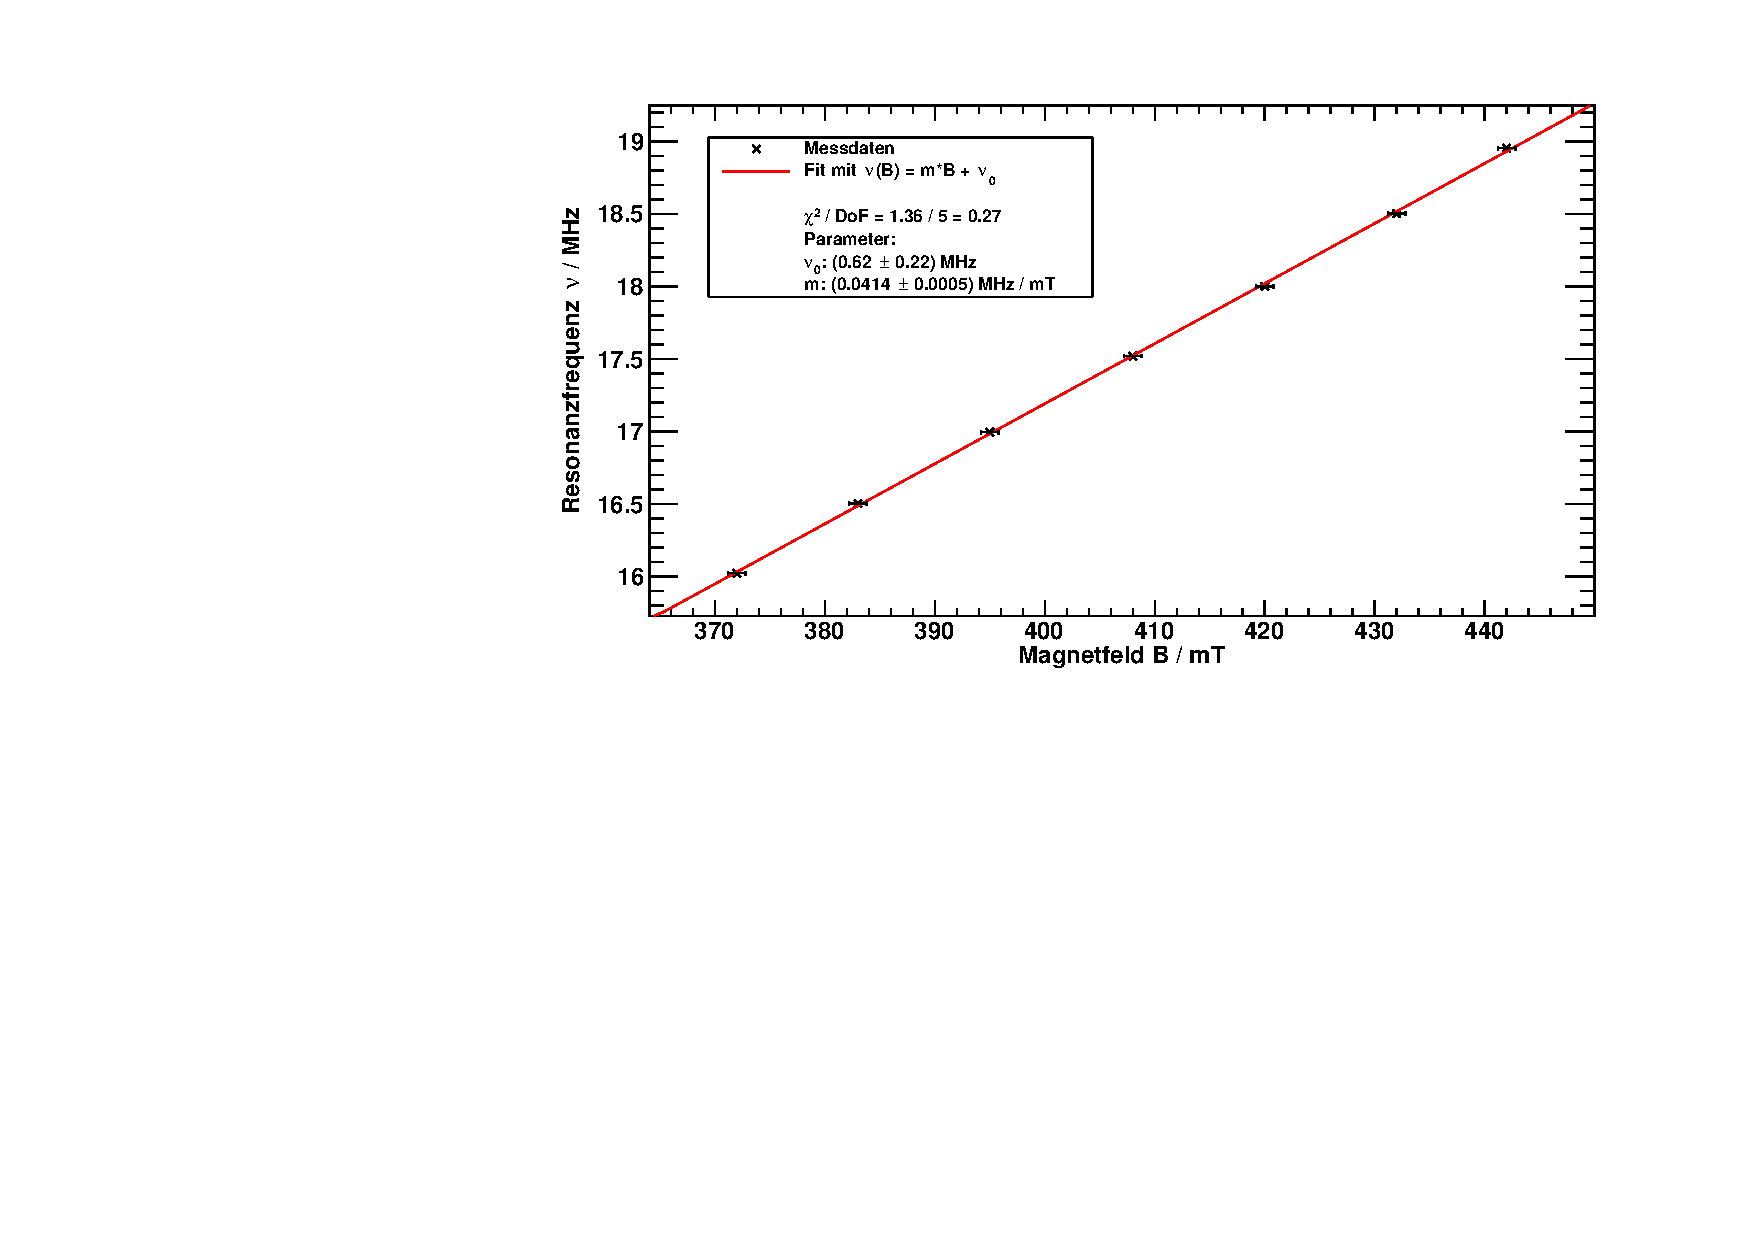
\includegraphics[width=\textwidth]{../img/03-H.pdf}
  \caption{Messungen der Resonanzfrequenzen $\nu$ an der Wasserstoffprobe für verschiedene Magnetfelder $B$.}
  \label{img:H}
\end{center}
\end{figure}
In \autoref{img:H} die Resonanzfrequenz $\nu$ über der verwendeten Magnetfeldstärke $B$ aufgetragen. Entsprechend \autoref{eq:nu} wurden 
die Daten mit 
\begin{equation}
  \nu(B) = m \cdot B
\end{equation}
gefittet.\footnote{Auf einen Achsenabschnitt wurde bewusst verzichtet, da die Stärken des Magnetfeldes sehr weit von 0 abweichen, und somit schon 
eine sehr kleine Abweichung der Steigung vom Erwartungswert zu einem großen Achsenabschnitt führt.} \\
Dem $\chi^2$-Wert ist ein linksseitiger p-Wert von 46\% zugeordnet. Dies zeigt, dass die Fehler richtig abgeschätzt wurden und das Modell 
die Messdaten korrekt beschreibt. \\
Man erhält für die Steigung
\begin{equation}
  m = (0.04295 \pm 0.00004)\,\frac{\text{MHz}}{\text{mT}}.
\end{equation}
Daraus lässt sich nach \autoref{eq:nu} durch Multiplikation mit dem Faktor $2 \pi$ das gyromagnetische Verhältnis von Wasserstoff $\gamma_H$ bestimmen. 
\begin{equation}
  \gamma_H = (270.0 \pm 0.3) \cdot 10^8\,\frac{1}{\text{s} \cdot \text{T}}
\end{equation}
Der relative Fehler beträgt:
\begin{equation}
  s_{\gamma_{H}, \text{rel}} = \frac{s_{\gamma H}}{\gamma_H} = 0.0009
\end{equation}
Er wird für die folgenden gyromagnetischen Verhältnisse benutzt.

\subsubsection{Berechnung von $\gamma_\text{Glykol}$ und $\gamma_\text{Teflon}$}
Mit \autoref{eq:nu} lässt sich das gyromagnetische Verhältnis von Glykol und Teflon bestimmen.
Man erhält
\begin{equation}
  \gamma_{\text{Glykol}} = (268.7 \pm 0.3) \cdot 10^8\,\frac{1}{\text{s} \cdot \text{T}}
\end{equation}
und
\begin{equation}
  \gamma_{\text{Teflon}} = (253.4 \pm 0.2) \cdot 10^8\,\frac{1}{\text{s} \cdot \text{T}} \ \, .
\end{equation}
Der Mittelwert $\overline{\gamma_H}$ für die beiden Messungen am Proton ($\gamma_{H}$ und $\gamma_{\text{Glykol}}$) beträgt
\begin{equation}
  \overline{\gamma_H} = (269.4 \pm 0.2) \cdot 10^8\,\frac{1}{\text{s} \cdot \text{T}}
\end{equation}
Die Literaturwerte\footnote{H: \url{http://physics.nist.gov/cgi-bin/cuu/Value?gammap}} 
\footnote{F: David R. Lide, ed., CRC Handbook of Chemistry
and Physics, Internet Version 2005, \url{http://www.hbcpnetbase.com}, CRC Press, Boca Raton, FL, 2005} lauten
\begin{equation}
  \gamma_H^\text{Lit} = 2.6752 \cdot 10^8 \,\frac{1}{\text{s} \cdot \text{T}}, \qquad 
  \gamma_F^\text{Lit} = 2.5166 \cdot 10^8 \,\frac{1}{\text{s} \cdot \text{T}}
\end{equation}
Die gemessenen Werte liegen beide ungefähr 1\% über den Literaturwerten. Dies deuted auf einen systematischen Fehler hin, zum Beispiel bei der 
Bestimmung des Magnetfeldes (äußere Magnetfelder, Drehung der Hallsonde).

\subsection{Berechnung des Kern-g-Faktors}
Mit \autoref{eq:gamma} können die Kern-g-Faktoren für die einzelnen Messungen berechnet werden.
Sie lauten
\begin{equation}
\begin{split}
g_{I,\text{H}}&= 5.634	\pm 0.005\\
g_{I,\text{Glykol}}&= 5.610	\pm 0.005\\
g_{I,\text{Teflon}}&= 5.301 \pm	0.005
\end{split}
\end{equation}
Auf einen Vergleich mit den Literaturwerten wird hier verzichtet, da nur das gyromagnetische Verhältnis mit bekannten Konstanten verrechnet wird. 
Dies gilt auch für den folgenden Abschnitt.


\subsection{Berechnung des kernmagnetischen Moments}
\autoref{eq:mu:z} liefert die kernmagnetischen Momente. Sie lauten
\begin{equation}
\begin{split}
\mu_{z,\text{H}}&= (1.4228	\pm 0.0013) \cdot 10^{-26}\,\frac{\text{J}}{\text{T}}\\
\mu_{z,\text{Glykol}}&= (1.4168	\pm 0.0013) \cdot 10^{-26}\,\frac{\text{J}}{\text{T}}\\
\mu_{z,\text{Teflon}}&= (1.3386	\pm 0.0012) \cdot 10^{-26}\,\frac{\text{J}}{\text{T}}
\end{split}
\end{equation}

